%\documentclass[aps,prstab,showpac,twocolumn]{revtex4-1}  
\documentclass[aps,prstab,onecolumn,preprint,nofootinbib]{revtex4-1}

\usepackage{graphicx}
\usepackage{epsfig}
\usepackage{subfigure}
\usepackage{fancyhdr}
\usepackage{color}
\usepackage{amsfonts}
\usepackage{amsmath}
\usepackage{amssymb}
\usepackage{dcolumn}
\usepackage{bm}
\usepackage{indentfirst}
\usepackage{rotating}
\usepackage{moreverb}

\setlength{\textwidth}{6.5in}
\setlength{\textheight}{8.5in}
\setlength{\topmargin}{0in}
\setlength{\oddsidemargin}{0.0in}
\setlength{\evensidemargin}{0.0in}
\setlength{\rightmargin}{0.0in}

\makeatletter

\begin{document}

\title{Studies of Particle Motions During Slow Resonant Extraction}
\author{Chong Shik Park, James Amundson, Leo Michelotti, and Vladimir Nagaslaev}
\affiliation{Fermi National Accelerator Laboratory, PO Box 500, Batavia, IL 60510}
\date{\today}

\begin{abstract}
We present here 
%The Mu2e experiment at Fermilab requires the acceleration and transport of intense proton beams, and the delivery of stable and uniform particle spills to the production target. To meet the experimental requirement, particles will be slowly extracted from the Delivery Ring to the external beamline. Using Synergia2, we have performed multi-particle tracking simulations of the third-integer resonant extraction in the Delivery Ring, including space charge effects as well as physical beamline elements and apertures. With a suitable ramp profile of tune-quadrupoles, we modeled a uniform spill structure. In order to minimize beam losses which are critical for efficient extractions, we have implemented a number of features, such as apertures in beamline elements, septum plane alignments. The RF Knockout (RFKO) technique, which excites particles transversely, is employed as a spill regulation system. Combined with a feedback system, it assists in fine-tuning the spill uniformity. Simulation studies have been carried out to optimize the RFKO feedback scheme, which will be helpful in designing the spill regulation system. 
\end{abstract}

\pacs{}
\maketitle

\setcounter{tocdepth}{5}

%\tableofcontents

%%%%%%%%%%%%%%%%%%%%%%%%%%%%%%%%%%%%%%%%%%%%%%%%%%%%%%%%%%%%%%%%%%%%%%
\section{\label{sec:intro}Introduction}

\clearpage
\section{\label{sec:bump}Phasespace Corrections with Dynamic Bumps}

In the previous paper, we discussed that a septum foil plane should be aligned with particles' $x^{\prime}$ coordinates when they are entering the field region of the septum. This alignment of the septum foil plane alogn with $x^{\prime}$s should be optimized to reduce particle losses due to crossing the plane from outside to inside the field region or vice versa. However, particles' angle coordinates are changing in time when a separatrix is being squeezed during an extraction period. 
Fig.~\ref{fig:bump0} shows unstable particles measured at the entrance of the first septum in normalized phase space coordinates for 4 different stages of extraction. Particle streams are entering the septum field region by crossing the vertical line (color:purple), and their coordinates are changing during the extraction.
Therefore, the alignment is only valid for a few turns at the beginning, and there will be misalignments of the septum foil plane with respect to $x^{\prime}$s later. These result in increasing of beam losses in time. Moreover, one can expect that an angular spread of extracted particles at the entrance of the septum will be large.

\begin{figure*}[tbh!]
  \begin{center}
    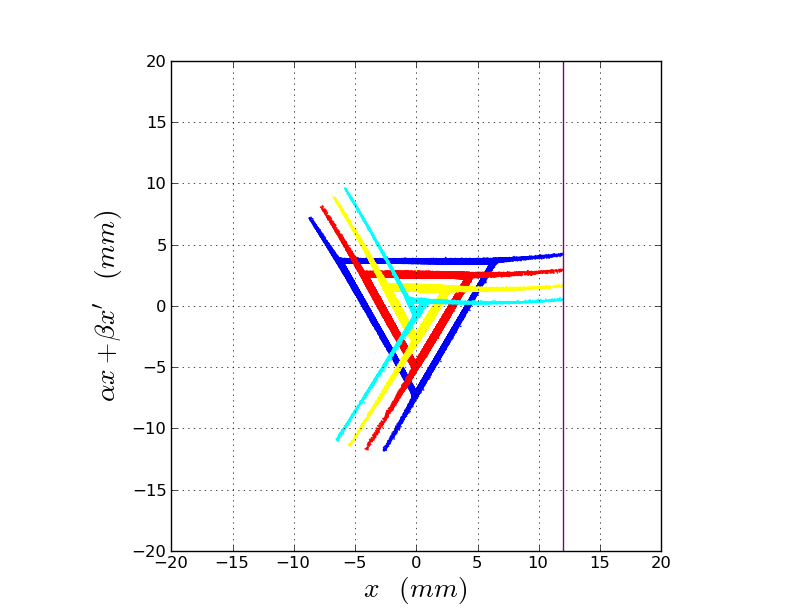
\includegraphics[width=.45\textwidth]{img/ufp.png}
    \caption{\label{fig:bump0}Normalized phase space plots of particles around separatrices.}
  \end{center}
\end{figure*}



\begin{figure*}[tbh!]
  \begin{center}
    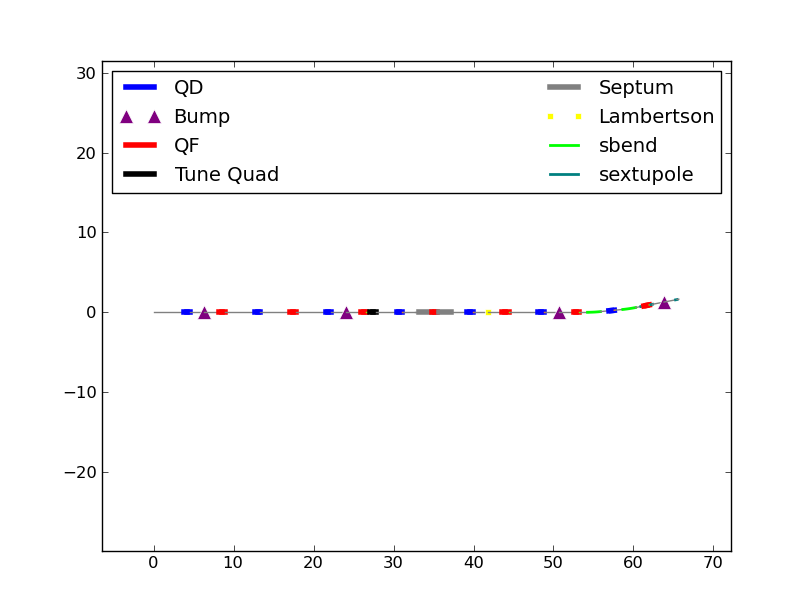
\includegraphics[width=.45\textwidth]{img/20140109-00.png}
    \caption{\label{fig:bump1}Schematic drawing of the external beamline with 4 dynamic bumps.}
  \end{center}
\end{figure*}


In order to mitigate these effects, orbit corrections are applied using 4 dynamic angle bumps. Fig.~\ref{fig:bump1} shows a schematic drawing of 4 dynamic bump locations in the extraction beamline. 2 bumps are located at the upstream of septa, and the other 2 are at the downstream. Upstream bumps kick particles so that outgoing particles' angles are aligned at the entrance end of the first septum during the entire extraction period. Then, downstream bumps will kick them back to original positions.

Using simple Bump strengths, $\theta_{i}$ for $i=1,2,3,4$, are given by
\begin{equation}
  \begin{split}
  \theta_{1}(t) & = \sqrt{\frac{\beta_{s}}{\beta_{1}}}
               \frac{\sin(\psi_{s} - \psi_{2})}
                    {\sin(\psi_{2} - \psi_{1})}
               \left( - \Delta x_{s}^{\prime} (t) \right),
  \;\;\;
  \theta_{2}(t) = \sqrt{\frac{\beta_{s}}{\beta_{2}}}
               \frac{\sin(\psi_{s} - \psi_{1})}
                    {\sin(\psi_{2} - \psi_{1})}
               \Delta x_{s}^{\prime} (t), \\
  \theta_{3}(t) & = \sqrt{\frac{\beta_{s}}{\beta_{3}}}
               \frac{\sin(\psi_{s} - \psi_{4})}
                    {\sin(\psi_{4} - \psi_{3})}
               \Delta x_{s}^{\prime} (t),
  \;\;\;\;\;\;\;\;\;\;
  \theta_{4}(t) = \sqrt{\frac{\beta_{s}}{\beta_{4}}}
               \frac{\sin(\psi_{s} - \psi_{3})}
                    {\sin(\psi_{4} - \psi_{3})}
               \left( - \Delta x_{s}^{\prime} (t) \right),
  \end{split}
\end{equation}
where $\beta_{i}$'s are betatron functions at the septum($s$) and bumps($1,2,3,4$), $\psi_{i}$'s are betatron phase advances, and $\Delta x^{\prime}_{s} (t)$ is required changes of angle coordinates at the septum as a function of time. Fig.~\ref{fig:bump2} shows changes of bump strengths in time. Since particles' angles are aligned to the initial angle, bump strengths are zero at the beginning and are maximum at the end of extraction.

\begin{figure*}[tbh!]
  \begin{center}
    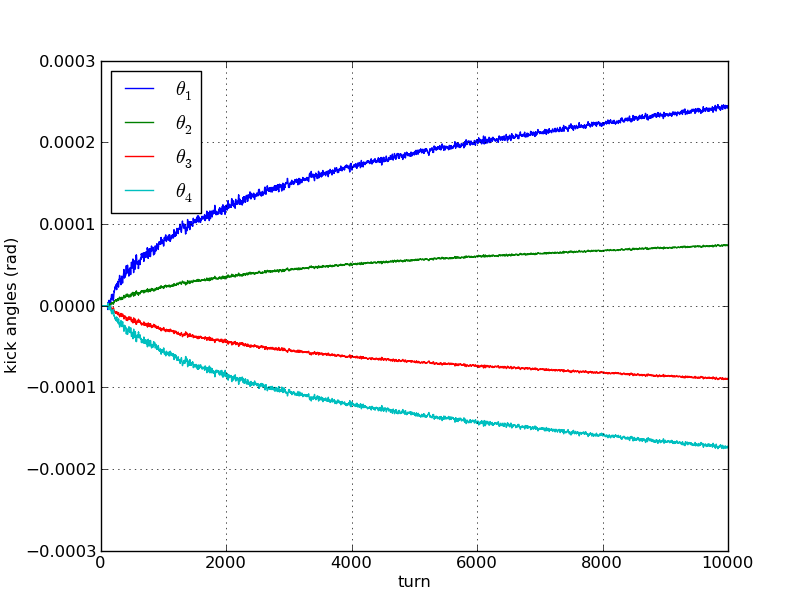
\includegraphics[width=.45\textwidth]{img/20140123-00.png}
    \caption{\label{fig:bump2}Strength changes of dynamic bumps in time.}
  \end{center}
\end{figure*}

Before applying dynamic bumps, phase space of circulating particles are centered at the origin as shown in Fig.~\ref{fig:bump0}. As the separatrix is squeezed by increaing tune-quad strengths, phase space areas are shrinking in time and outgoing branches 


\begin{figure*}[tbh!]
  \begin{center}
    \subfigure[Without Dynamic Bumps]{
      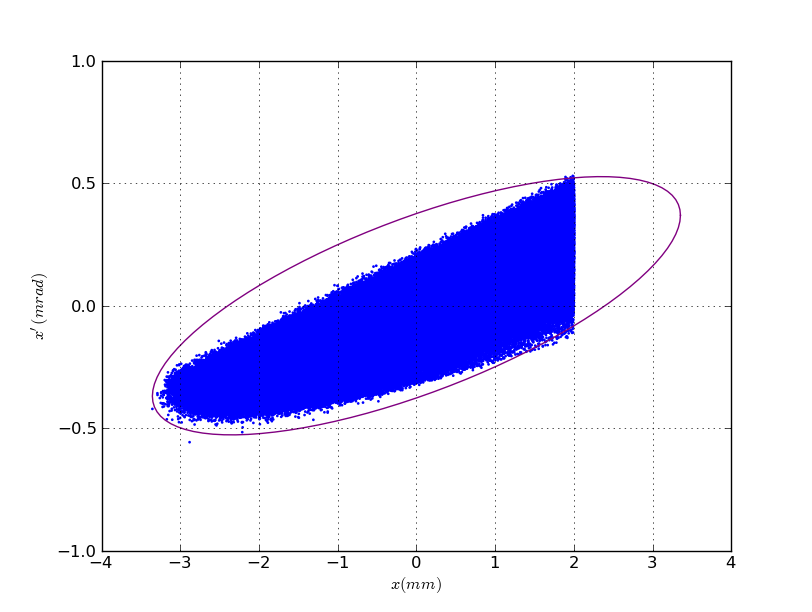
\includegraphics[width=.45\textwidth]{img/20140206-02.png}
      \label{fig:bumpps3}}
    \subfigure[With Dynamic Bumps]{
      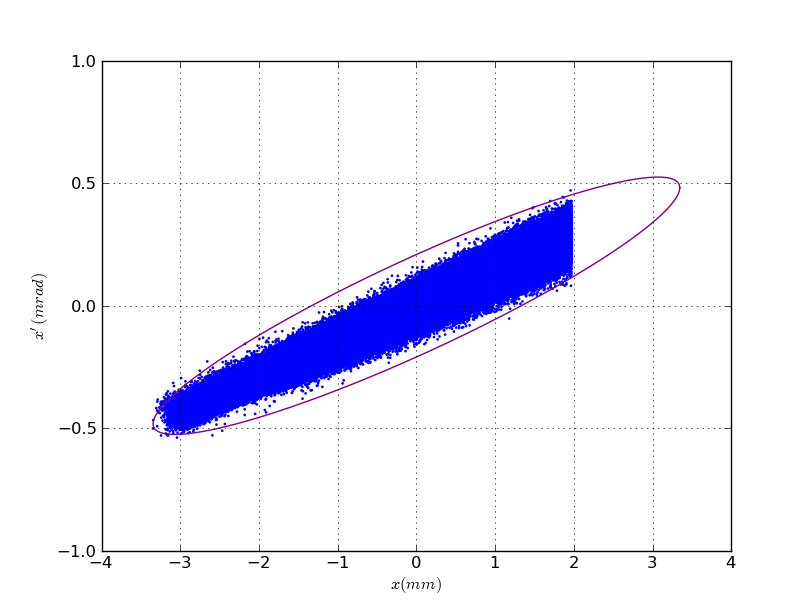
\includegraphics[width=.45\textwidth]{img/20140206-03.png}
      \label{fig:bumpps4}}
    \caption{\label{fig:bump4}Footprints of extracted particles with/without dynamic bumps.}
  \end{center}
\end{figure*}

\begin{figure*}[tbh!]
  \begin{center}
    \subfigure[Without Dynamic Bumps]{
      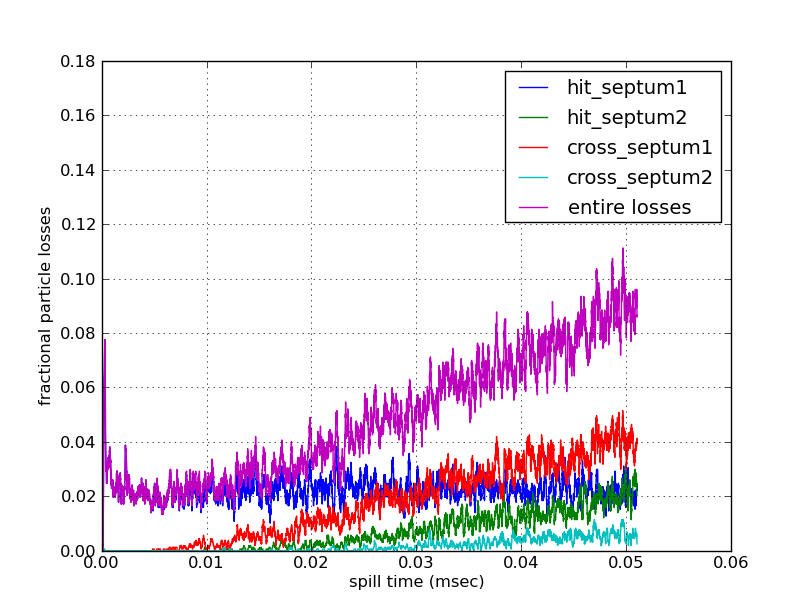
\includegraphics[width=.45\textwidth]{img/20140203-06.png}
      \label{fig:bumploss1}}
    \subfigure[With Dynamic Bumps]{
      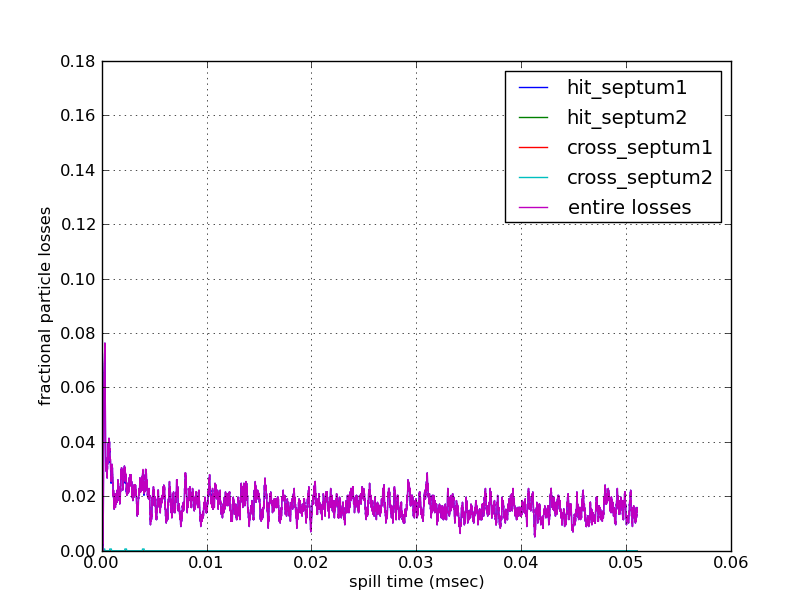
\includegraphics[width=.45\textwidth]{img/20140203-07.png}
      \label{fig:bumploss2}}
    \caption{\label{fig:bump5}Particle losses in time with/without dynamic bumps.}
  \end{center}
\end{figure*}

\section{\label{sec:loss}Tracking of Particle Losses}



\section{\label{sec:emit}Emittance Growth Rates with RFKO Beam Heating}

\section{\label{sec:rfko}RFKO Beam Distribution Function}

\section{\label{sec:arrival}Arrival Time Distribution}

\section{\label{sec:conclusion}Conclusion}

\section{\label{thanks}Acknowledgments}

\begin{thebibliography}{77}


\end{thebibliography}

\end{document}
